% Options for packages loaded elsewhere
\PassOptionsToPackage{unicode}{hyperref}
\PassOptionsToPackage{hyphens}{url}
%
\documentclass[
  man,floatsintext]{apa7}
\usepackage{amsmath,amssymb}
\usepackage{lmodern}
\usepackage{iftex}
\ifPDFTeX
  \usepackage[T1]{fontenc}
  \usepackage[utf8]{inputenc}
  \usepackage{textcomp} % provide euro and other symbols
\else % if luatex or xetex
  \usepackage{unicode-math}
  \defaultfontfeatures{Scale=MatchLowercase}
  \defaultfontfeatures[\rmfamily]{Ligatures=TeX,Scale=1}
\fi
% Use upquote if available, for straight quotes in verbatim environments
\IfFileExists{upquote.sty}{\usepackage{upquote}}{}
\IfFileExists{microtype.sty}{% use microtype if available
  \usepackage[]{microtype}
  \UseMicrotypeSet[protrusion]{basicmath} % disable protrusion for tt fonts
}{}
\makeatletter
\@ifundefined{KOMAClassName}{% if non-KOMA class
  \IfFileExists{parskip.sty}{%
    \usepackage{parskip}
  }{% else
    \setlength{\parindent}{0pt}
    \setlength{\parskip}{6pt plus 2pt minus 1pt}}
}{% if KOMA class
  \KOMAoptions{parskip=half}}
\makeatother
\usepackage{xcolor}
\usepackage{graphicx}
\makeatletter
\def\maxwidth{\ifdim\Gin@nat@width>\linewidth\linewidth\else\Gin@nat@width\fi}
\def\maxheight{\ifdim\Gin@nat@height>\textheight\textheight\else\Gin@nat@height\fi}
\makeatother
% Scale images if necessary, so that they will not overflow the page
% margins by default, and it is still possible to overwrite the defaults
% using explicit options in \includegraphics[width, height, ...]{}
\setkeys{Gin}{width=\maxwidth,height=\maxheight,keepaspectratio}
% Set default figure placement to htbp
\makeatletter
\def\fps@figure{htbp}
\makeatother
\setlength{\emergencystretch}{3em} % prevent overfull lines
\providecommand{\tightlist}{%
  \setlength{\itemsep}{0pt}\setlength{\parskip}{0pt}}
\setcounter{secnumdepth}{-\maxdimen} % remove section numbering
% Make \paragraph and \subparagraph free-standing
\ifx\paragraph\undefined\else
  \let\oldparagraph\paragraph
  \renewcommand{\paragraph}[1]{\oldparagraph{#1}\mbox{}}
\fi
\ifx\subparagraph\undefined\else
  \let\oldsubparagraph\subparagraph
  \renewcommand{\subparagraph}[1]{\oldsubparagraph{#1}\mbox{}}
\fi
\ifLuaTeX
\usepackage[bidi=basic]{babel}
\else
\usepackage[bidi=default]{babel}
\fi
\babelprovide[main,import]{english}
% get rid of language-specific shorthands (see #6817):
\let\LanguageShortHands\languageshorthands
\def\languageshorthands#1{}
% Manuscript styling
\usepackage{upgreek}
\captionsetup{font=singlespacing,justification=justified}

% Table formatting
\usepackage{longtable}
\usepackage{lscape}
% \usepackage[counterclockwise]{rotating}   % Landscape page setup for large tables
\usepackage{multirow}		% Table styling
\usepackage{tabularx}		% Control Column width
\usepackage[flushleft]{threeparttable}	% Allows for three part tables with a specified notes section
\usepackage{threeparttablex}            % Lets threeparttable work with longtable

% Create new environments so endfloat can handle them
% \newenvironment{ltable}
%   {\begin{landscape}\centering\begin{threeparttable}}
%   {\end{threeparttable}\end{landscape}}
\newenvironment{lltable}{\begin{landscape}\centering\begin{ThreePartTable}}{\end{ThreePartTable}\end{landscape}}

% Enables adjusting longtable caption width to table width
% Solution found at http://golatex.de/longtable-mit-caption-so-breit-wie-die-tabelle-t15767.html
\makeatletter
\newcommand\LastLTentrywidth{1em}
\newlength\longtablewidth
\setlength{\longtablewidth}{1in}
\newcommand{\getlongtablewidth}{\begingroup \ifcsname LT@\roman{LT@tables}\endcsname \global\longtablewidth=0pt \renewcommand{\LT@entry}[2]{\global\advance\longtablewidth by ##2\relax\gdef\LastLTentrywidth{##2}}\@nameuse{LT@\roman{LT@tables}} \fi \endgroup}

% \setlength{\parindent}{0.5in}
% \setlength{\parskip}{0pt plus 0pt minus 0pt}

% Overwrite redefinition of paragraph and subparagraph by the default LaTeX template
% See https://github.com/crsh/papaja/issues/292
\makeatletter
\renewcommand{\paragraph}{\@startsection{paragraph}{4}{\parindent}%
  {0\baselineskip \@plus 0.2ex \@minus 0.2ex}%
  {-1em}%
  {\normalfont\normalsize\bfseries\itshape\typesectitle}}

\renewcommand{\subparagraph}[1]{\@startsection{subparagraph}{5}{1em}%
  {0\baselineskip \@plus 0.2ex \@minus 0.2ex}%
  {-\z@\relax}%
  {\normalfont\normalsize\itshape\hspace{\parindent}{#1}\textit{\addperi}}{\relax}}
\makeatother

% \usepackage{etoolbox}
\makeatletter
\patchcmd{\HyOrg@maketitle}
  {\section{\normalfont\normalsize\abstractname}}
  {\section*{\normalfont\normalsize\abstractname}}
  {}{\typeout{Failed to patch abstract.}}
\patchcmd{\HyOrg@maketitle}
  {\section{\protect\normalfont{\@title}}}
  {\section*{\protect\normalfont{\@title}}}
  {}{\typeout{Failed to patch title.}}
\makeatother

\usepackage{xpatch}
\makeatletter
\xapptocmd\appendix
  {\xapptocmd\section
    {\addcontentsline{toc}{section}{\appendixname\ifoneappendix\else~\theappendix\fi\\: #1}}
    {}{\InnerPatchFailed}%
  }
{}{\PatchFailed}
\usepackage{lineno}

\linenumbers
\usepackage{csquotes}
\usepackage{amsmath}
\usepackage[labelformat=empty]{caption}
\usepackage{caption}
\usepackage[extra]{tipa}
\renewcommand{\topfraction}{1}
\renewcommand{\bottomfraction}{1}
\renewcommand{\textfraction}{.1}
\renewcommand{\floatpagefraction}{1}
\setcounter{topnumber}{9}
\setcounter{bottomnumber}{9}
\setcounter{totalnumber}{20}
\setcounter{dbltopnumber}{9}
\renewcommand{\thefigure}{S\arabic{figure}}
\makeatletter
\renewcommand{\paragraph}{\@startsection{paragraph}{4}{\parindent}%
  {0\baselineskip \@plus 0.2ex \@minus 0.2ex}%
  {-1em}%
  {\normalfont\normalsize\bfseries\typesectitle}}

\renewcommand{\subparagraph}[1]{\@startsection{subparagraph}{5}{1em}%
  {0\baselineskip \@plus 0.2ex \@minus 0.2ex}%
  {-\z@\relax}%
  {\normalfont\normalsize\bfseries\itshape\hspace{\parindent}{#1}\textit{\addperi}}{\relax}}
\makeatother

\ifLuaTeX
  \usepackage{selnolig}  % disable illegal ligatures
\fi
\IfFileExists{bookmark.sty}{\usepackage{bookmark}}{\usepackage{hyperref}}
\IfFileExists{xurl.sty}{\usepackage{xurl}}{} % add URL line breaks if available
\urlstyle{same} % disable monospaced font for URLs
\hypersetup{
  pdftitle={Supplemental Materials},
  pdfauthor={Rachel Ka-Ying Tsui1, Jessica E. Kosie2, Laia Fibla1, Casey Lew-Williams2, \& Krista Byers-Heinlein1},
  pdflang={en-EN},
  hidelinks,
  pdfcreator={LaTeX via pandoc}}

\title{Supplemental Materials}
\author{Rachel Ka-Ying Tsui\textsuperscript{1}, Jessica E. Kosie\textsuperscript{2}, Laia Fibla\textsuperscript{1}, Casey Lew-Williams\textsuperscript{2}, \& Krista Byers-Heinlein\textsuperscript{1}}
\date{}


\shorttitle{Tablet Switch}

\authornote{

Correspondence concerning this article should be addressed to Rachel Ka-Ying Tsui, Department of Psychology, 7141 Sherbrooke St.~West, Montreal, QC, Canada, H2T1V2. Rachel Ka-Ying Tsui is now at Laboratory for Language Development, RIKEN Center for Brain Science, 2-1 Hirosawa, Wako-shi, Saitama, Japan, 351-0198. Email: \href{mailto:rachelkytsui@gmail.com}{\nolinkurl{rachelkytsui@gmail.com}}. Experiment material, analysis scripts, data set, and supplemental materials are available at \url{https://osf.io/8vk3b/}.. E-mail: \href{mailto:rachelkytsui@gmail.com}{\nolinkurl{rachelkytsui@gmail.com}}

}

\affiliation{\vspace{0.5cm}\textsuperscript{1} Concordia University\\\textsuperscript{2} Princeton University}

\begin{document}
\maketitle

\captionsetup[table]{labelformat=empty}

\hypertarget{detailed-descriptive-statistics-of-the-childrens-proficiency-scores}{%
\subsection{Detailed descriptive statistics of the children's proficiency scores}\label{detailed-descriptive-statistics-of-the-childrens-proficiency-scores}}

As mentioned in the main paper, out of the 49 children with proficiency data: 14 children had equal comprehension proficiency in both languages (8 French--English, 6 Spanish--English); 17 children were more proficient in English comprehension than French/Spanish (12 French--English, 5 Spanish--English); and 18 children were more proficient in French/Spanish than in English (7.10 French--English, 6.50 Spanish--English). Proficiency data was missing from 1 French--English and 3 Spanish--English children. Table S1 lists the detailed descriptive statistics of the proficiency scores.

\begin{figure}[H]

{\centering 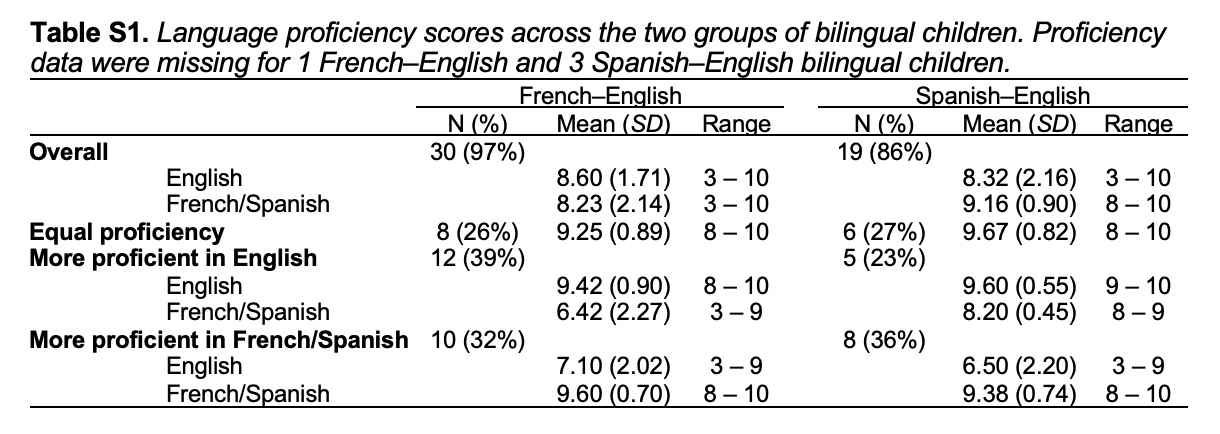
\includegraphics[width=1\linewidth]{/Users/racheltsui/Documents/GitHub/Bilingual-Families-Project_TabletSwitch/analysis/paper/figure/TableS1} 

}

\end{figure}

A linear regression model with proficiency score as the dependent variable was run to compare proficiency scores between the French--English and Spanish--English bilinguals. In the linear regression model, fixed effects included language community (French--English vs.~Spanish--English) and language (English vs.~French/Spanish), as well as their interaction\footnote{We tried running a linear mixed-effects model with a random intercept for participants; however, the model returned a singular fit.}:

proficiency \textasciitilde{} language * lang\_community

\noindent We found no significant effect of language, language community, nor their interaction (\emph{p}s \textgreater{} 0.11. Therefore, there was no significant difference between the French--English and Spanish--English children in terms of their proficiency in English or their proficiency in the other language (i.e., French for the French--English children and Spanish for the Spanish--English children).

\hypertarget{exploratory-analysis-of-the-main-paper}{%
\subsection{Exploratory analysis of the main paper}\label{exploratory-analysis-of-the-main-paper}}

In the main paper, we reported the preregistered analyses on accuracy --- our primary dependent variable in determining bilingual children's word learning in touching the labeled target object on each test trial. In this supplemental materials, we report two preregistered exploratory analyses: (1) looking at the effect of age, (2) using response time as the dependent variable, and an additional analysis on the effect of language proficiency.

\hypertarget{effect-of-age}{%
\subsubsection{Effect of age}\label{effect-of-age}}

Our accuracy analysis revealed that bilingual children in both communities successfully learned the novel words regardless of the language switching patterns used during the learning blocks. As previous research has shown that children's ability to learn words may improve with age (e.g., Read et al., 2021; Scaff et al., 2022), in our preregistration we also expected older children to show a greater accuracy than younger children. Therefore, we additionally compared models with and without age as a predictor variable. Bilingual children's age in months was scaled and centered for ease of interpretation. The final model specification was:

accuracy \textasciitilde{} condition * lang\_community * age\_in\_months + (1 + condition\textbar participant) + (1\textbar item)

\noindent When added to the model, neither the main effect nor interactions with age were significant (all \emph{p}s \textgreater{} 0.30; see Table S2 for the coefficient estimates from this model). Moreover, a model comparison with and without age as a variable indicated no significant improvement in model fit, \(\chi^2\)(4) = 2.26, \emph{p} = 0.69. Overall, the pattern in this model was consistent with the main accuracy analysis reported in the paper where there was no significant difference in terms of condition or language community, suggesting that bilingual children successfully learned the novel words regardless of age.

\begin{table}[H]

\begin{center}
\begin{threeparttable}

\caption{\label{tab:unnamed-chunk-6}Table S2. Coefficient estimates from the logistic mixed-effects models predicting accuracy in the test blocks with age\_in\_months as an additional fixed effect.}

\begin{tabular}{lcccc}
\toprule
 & Estimate & $SE$ & $z$ & $p$\\
\midrule
Intercept & 1.240 & 0.221 & 5.610 & <.001\\
condition & 0.118 & 0.307 & 0.386 & 0.7\\
lang\_community & 0.237 & 0.384 & 0.618 & 0.537\\
age\_in\_months & 0.109 & 0.181 & 0.604 & 0.546\\
condition * lang\_community & 0.020 & 0.592 & 0.034 & 0.973\\
condition * age\_in\_months & 0.088 & 0.294 & 0.298 & 0.766\\
lang\_community * age\_in\_months & -0.256 & 0.361 & -0.709 & 0.479\\
condition * lang\_community * age\_in\_months & 0.609 & 0.590 & 1.030 & 0.302\\
\bottomrule
\end{tabular}

\end{threeparttable}
\end{center}

\end{table}

\hypertarget{response-time}{%
\subsubsection{Response Time}\label{response-time}}

In addition to accuracy, we explored response time on each correctly-responded test trial as a dependent variable; a total of 853 correct trials were included in this analysis. The decision to use response time as an additional measure was driven by a possibility that this measure might be able to better capture more individual variability in terms of the speed of children's lexical comprehension performance, since children were generally very accurate in the task. Moreover, response time may also be more sensitive to age effects, as children answer more quickly as they get older and gain more expertise with language (Scaff et al., 2022). On average, French--English bilingual children had a mean response time of 1997ms in the \emph{immediate-translation} condition (\(SD\) = 1064.2; range = 451.86 -- 5130.5) and 1788ms in the \emph{one-language-at-a-time} condition (\(SD\) = 880.09; range = 339.33 -- 4323.33). On the other hand, Spanish--English bilingual children had a mean response time of 2620ms in the \emph{immediate-translation} condition (\(SD\) = 1353.25; range = 764.33 -- 6166.5) and 2303ms in the \emph{one-language-at-a-time} condition (\(SD\) = 1455.58; range = 457.25 -- 5550.6).

A linear mixed-effects model was run on response time. To correct for issues of non-normality, raw response time was log-transformed. Condition, language community, and age, as well as their interactions, were entered as fixed effects in the model; a random slope of condition by participant and a random intercept of stimulus item were also entered:

log\_rt \textasciitilde{} condition * lang\_community * age\_in\_month + (1 + condition\textbar participant) + (1\textbar item)

\noindent The coefficient estimates from this model are shown in Table S3 and Figure S1 visualizes this model. The only terms that approached significance was the three-way interaction. Following up on this three-way interaction, separate linear mixed-effects analyses were run for the French--English bilinguals and the Spanish--English bilinguals. The models revealed that the effect of age approached significance in the \emph{immediate-translation} condition for the French--English bilinguals (Estimate = -0.19, SE = 0.10, t = -1.76, \emph{p} = 0.09), suggesting that the reaction time for French--English bilinguals decreased significantly in the \emph{immediate-translation} condition across age. However, the effect of age was not significant for the Spanish--English bilinguals (Estimate = 0.02, SE = 0.11, t = 0.13, \emph{p} = 0.90). Moreover, we found no significant interaction across age between the two conditions in either group of bilinguals. Overall, similar to the patterns reported in the first set of analysis on accuracy, we did not observe any significant difference in terms of condition or language community, nor in their interaction. Therefore, consistent with the accuracy analysis, bilingual children in both communities performed similarly in word learning across both the \emph{immediate-translation} and \emph{one-language-at-a-time} conditions.

\begin{table}[tbp]

\begin{center}
\begin{threeparttable}

\caption{\label{tab:unnamed-chunk-9}Table S3. Coefficient estimates from the linear mixed-effects model predicting log-transformed response time in the test blocks.}

\begin{tabular}{lcccc}
\toprule
 & Estimate & $SE$ & $t$ & $p$\\
\midrule
Intercept & 7.220 & 0.076 & 94.600 & <.001\\
condition & -0.098 & 0.079 & -1.250 & 0.22\\
lang\_community & 0.164 & 0.146 & 1.130 & 0.265\\
age\_in\_months & -0.094 & 0.071 & -1.330 & 0.189\\
condition * lang\_community & -0.122 & 0.157 & -0.775 & 0.443\\
condition * age\_in\_months & 0.010 & 0.078 & 0.125 & 0.901\\
lang\_community * age\_in\_months & 0.072 & 0.142 & 0.505 & 0.616\\
condition * lang\_community * age\_in\_months & -0.281 & 0.157 & -1.790 & 0.08\\
\bottomrule
\end{tabular}

\end{threeparttable}
\end{center}

\end{table}

\begin{figure}

{\centering 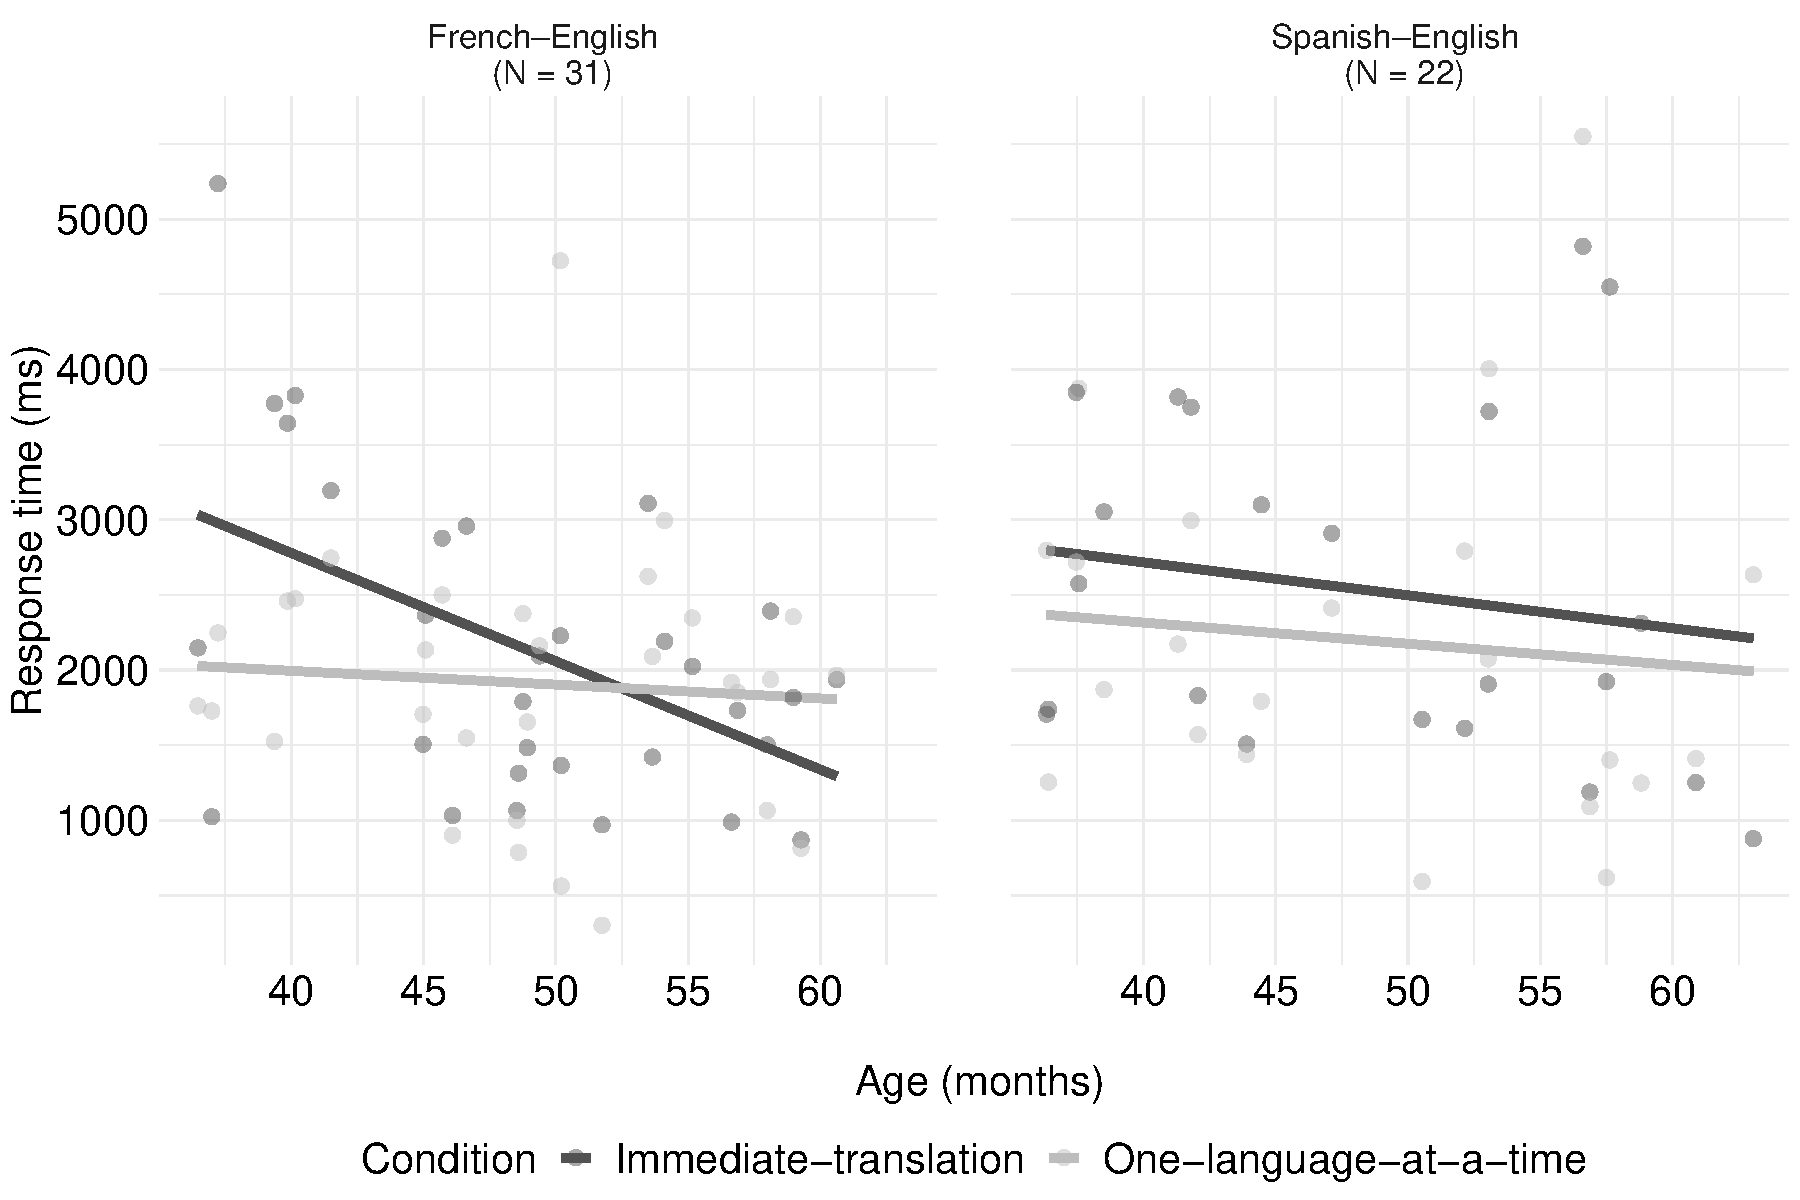
\includegraphics[width=0.9\linewidth]{TabletSwitch_supplemental_files/figure-latex/FigureS1-1} 

}

\caption{Response time by condition, language community, and age in the test block. Individual dots plot the data from each individual participant.}\label{fig:FigureS1}
\end{figure}

\hypertarget{language-proficiency}{%
\subsubsection{Language Proficiency}\label{language-proficiency}}

In addition to the preregistered analyses, we explored the effect of language proficiency on bilingual children's learning of the novel cross-language words. Previous research has revealed mixed evidence as to whether language proficiency interacts with bilingual children's word learning ability during different types of bilingual book reading sessions (e.g., Brouillard et al., 2022; Read et al., 2021). Therefore, it is plausible that language proficiency may have an effect on how bilingual children learn from different language switching patterns.

Building upon the logistic mixed-effects model used in the main accuracy analysis, we added a variable of proficiency score to the model. This created a continuous variable with the caregiver-reported proficiency rating in each language, which we used to predict children's performance on trials in that same language. In this analysis, we excluded data from one French--English and three Spanish--English children participants who were missing their proficiency information; data from 30 French--English and 19 Spanish--English children remained in the analysis. The initial specification was:

accuracy \textasciitilde{} condition * lang\_community * proficiency + (1 + condition\textbar participant) + (1\textbar item)

However, as the initial model did not converge, we first removed the random slope for condition and the random intercept for item. Moreover, since we did not find any significant difference between the two communities in the main accuracy analysis, we performed a model comparison between the model with language communities and the one without. This comparison also indicated no significant improvement in model fit, \(\chi^2\)(4) = 4.74, \(p\) = 0.32, so we further pruned the effect of language community from the model. Therefore, the final model was:

accuracy \textasciitilde{} condition * proficiency + (1\textbar participant)

\noindent The coefficient estimates from this model are shown in Table S4 and Figure S2 visualizes this model. Similar to the main analysis, no significant difference between conditions was found. Moreover, we did not observe any significant effect of language proficiency. As can be seen in Figure S2, the level of proficiency did not hugely impact children' accuracy in our experiment. Note that we also ran another model including all the children who participated in our experiment (i.e., including those who did not initially meet our language proficiency criteria; please refer to the section below for the detailed statistics).

\begin{table}[tbp]

\begin{center}
\begin{threeparttable}

\caption{\label{tab:unnamed-chunk-11}Table S4. Coefficient estimates from the logistic mixed-effects model predicting accuracy in the test blocks with language proficiency scores.}

\begin{tabular}{lcccc}
\toprule
 & Estimate & $SE$ & $z$ & $p$\\
\midrule
Intercept & 0.533 & 0.468 & 1.140 & 0.255\\
condition & 0.652 & 0.693 & 0.940 & 0.347\\
proficiency & 0.076 & 0.051 & 1.480 & 0.138\\
condition * proficiency & -0.064 & 0.079 & -0.802 & 0.423\\
\bottomrule
\end{tabular}

\end{threeparttable}
\end{center}

\end{table}

\begin{figure}

{\centering 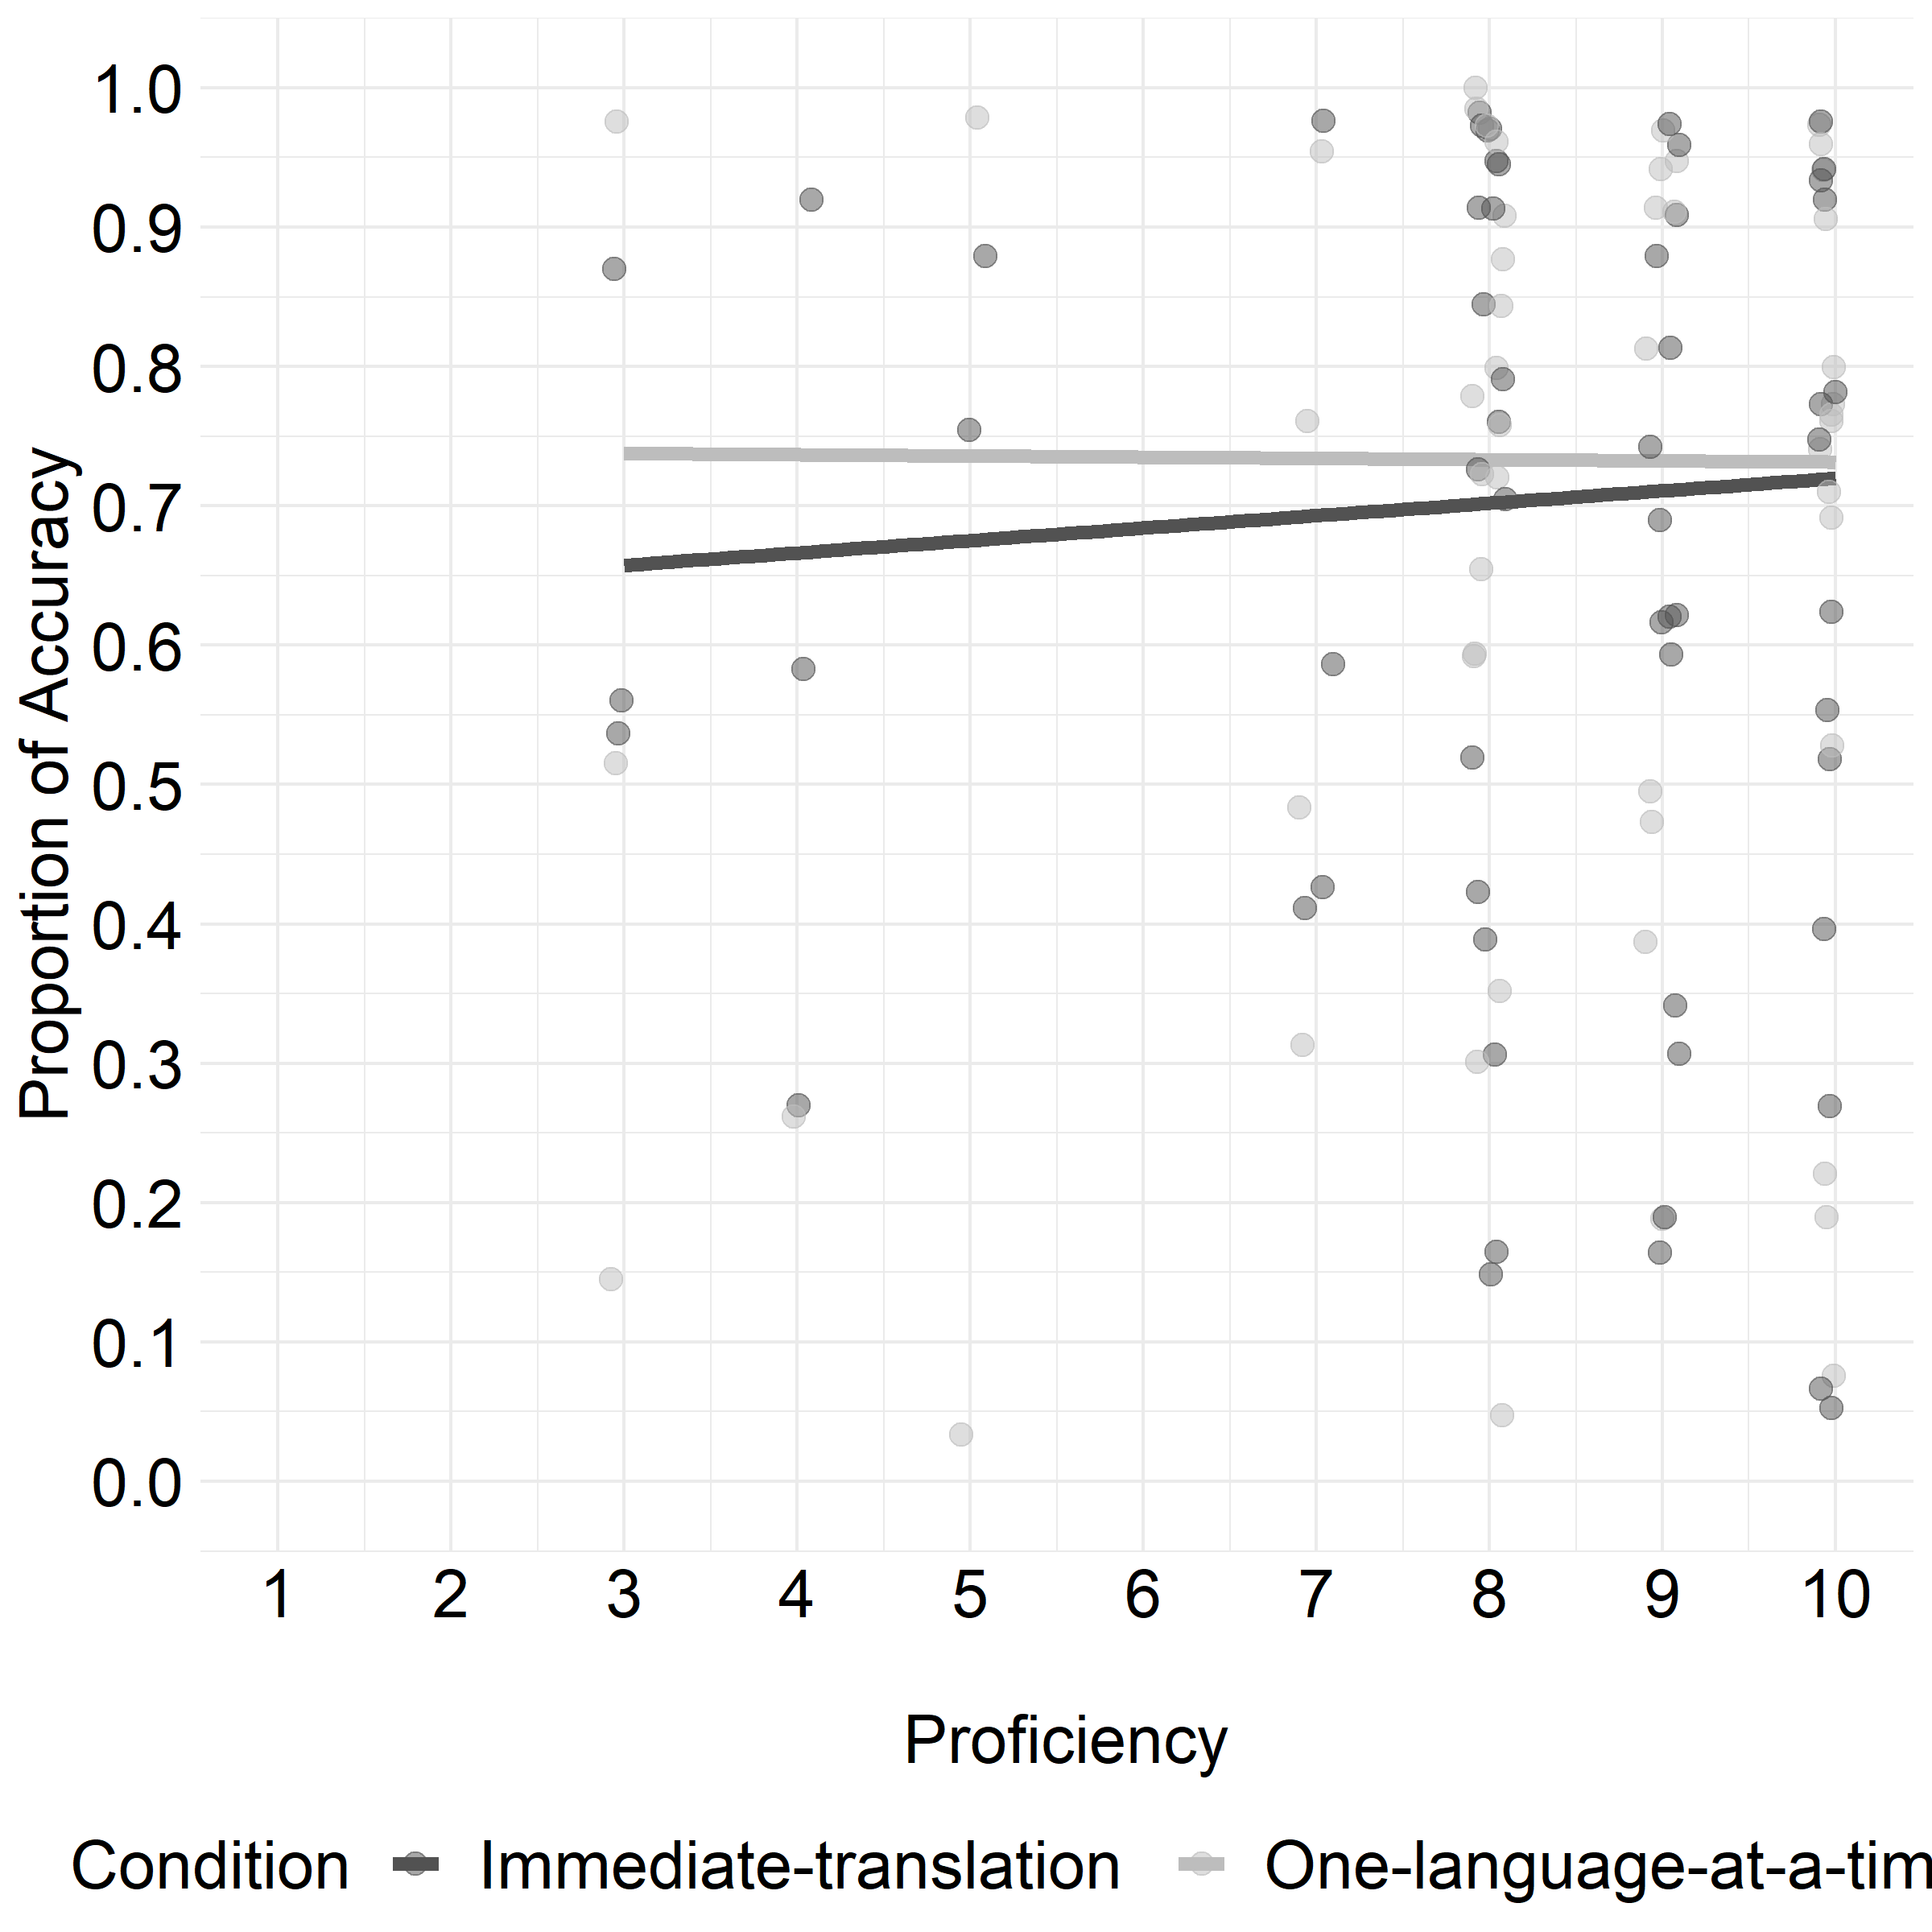
\includegraphics[width=0.5\linewidth]{TabletSwitch_supplemental_files/figure-latex/FigureS2-1} 

}

\caption{Proportion of accuracy by condition and language proficiency in the test blocks. Individual dots plot the data from each individual participant.}\label{fig:FigureS2}
\end{figure}

\hypertarget{supplemental-analysis-using-the-preregistered-exclusion-criteria}{%
\subsection{Supplemental analysis using the preregistered exclusion criteria}\label{supplemental-analysis-using-the-preregistered-exclusion-criteria}}

Analyses reported in the main paper deviated from the preregistered language exclusion criteria, as it resulted in exclusion of a higher than anticipated number of children and thus led to a smaller sample size and decreased statistical power. For transparency, this supplemental material reports the analyses using the more stringent preregistered exclusion criteria.

Following the preregistered language exclusion criteria, a total of 10 French--English and 12 Spanish--English children were excluded. When additional exclusion criteria were applied (see participants section in the main paper), the remaining sample consisted of 22 French--English children (13 girls; Mean age = 4.04 years, \(SD\) = 0.56, range = 3.04 -- 4.94) and 14 Spanish--English children (7 girls; Mean age = 4.21 years, \(SD\) = 0.75, range = 3.03 -- 5.26).

\begin{figure}[H]

{\centering 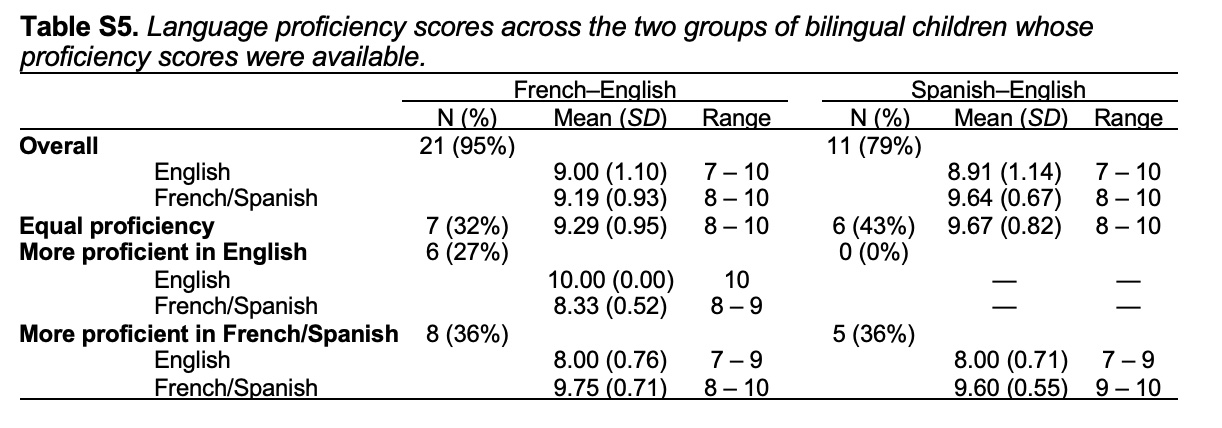
\includegraphics[width=1\linewidth]{/Users/racheltsui/Documents/GitHub/Bilingual-Families-Project_TabletSwitch/analysis/paper/figure/TableS5} 

}

\end{figure}

Language proficiency information was missing for 1 French--English and 3 Spanish--English children; 13 children had equal comprehension proficiency in both languages (7 French--English, 6 Spanish--English); 6 French--English children were more proficient in English comprehension than French/Spanish; and 13 children were more proficient in French/Spanish than in English (8 French--English, 5 Spanish--English). Table S5 contains descriptive statistics of the proficiency scores. We also ran a linear regression model with proficiency score as the dependent variable to compare proficiency scores between the French--English and Spanish--English bilinguals\footnote{In the linear regression model with proficiency scores as the dependent variable, fixed effects included language community (French--English vs.~Spanish--English) and language (English vs.~French/Spanish), as well as their interaction.}. There was no significant effect of language, language community, nor their interaction (\(p\)s \textgreater{} 0.30). Similar to the sample reported in the main paper, there was no significant difference between the French--English and Spanish--English children in terms of their proficiency in English as well as their proficiency in the other language (i.e., French for the French--English children and Spanish for the Spanish--English children). In this more restricted data set, 68\% of the mothers in Montreal and 64\% of the mothers in New Jersey had completed a university degree or higher.

In the following analyses, we followed the same procedure as in the main paper, where we first explored the preregistered analyses with proportion of accuracy as the dependent variable and then performed exploratory analyses: (1) on the effect of age, (2) with response time as the dependent variable, and (3) the effect of proficiency.

\hypertarget{accuracy}{%
\subsubsection{Accuracy}\label{accuracy}}

\hypertarget{familiar-word-block}{%
\paragraph{Familiar word block}\label{familiar-word-block}}

French--English bilingual children showed a mean accuracy of 0.98 in the familiar English-word trials (\(SD\) = 0.05; range = 0.83 -- 1) and 0.98 in the familiar French-word trials (\(SD\) = 0.05; range = 0.83 -- 1). Meanwhile, Spanish--English bilingual children showed a mean accuracy of 1 in the familiar English-word trials (\(SD\) = 0) and 1 in the familiar Spanish-word trials (\(SD\) = 0). As children's performance was almost at ceiling with little variance, it was not possible to fit the logistic mixed-effects model to compare performance across the two communities. On the other hand, this near-ceiling accuracy also suggests that our preregistered exclusion criteria could be too stringent such that only children with nearly perfect accuracy were included in the analyses.

\hypertarget{test-blocks}{%
\paragraph{Test blocks}\label{test-blocks}}

On average, French--English bilingual children showed a mean accuracy of 0.72 in the \emph{immediate-translation} condition (\(SD\) = 0.25; range = 0.17 -- 1) and 0.68 in the \emph{one-language-at-a-time} condition (\(SD\) = 0.27; range = 0 -- 1). On the other hand, Spanish--English bilingual children showed a mean accuracy of 0.76 in the \emph{immediate-translation} condition (\(SD\) = 0.23; range = 0.25 -- 1) and 0.7 in the \emph{one-language-at-a-time} condition (\(SD\) = 0.24; range = 0.33 -- 1). Separate one-sample t-tests were run on the proportion of accuracy in each condition per community, and confirmed that children from both communities learned the novel words in each condition significantly above the at-chance level of 0.50 (ps \textless{} .01)\footnote{For the French--English bilinguals, they performed significantly above the at-chance level in the \emph{immediate-translation} condition (\(t\)(21) = 4.01, \(p < .001\)) and the \emph{one-language-at-a-time} condition (\(t\)(21) = 3.14, \(p = .002\)). Likewise, the Spanish--English bilinguals performed significantly above the at-chance level in the \emph{immediate-translation} condition (\(t\)(13) = 4.24, \(p < .001\)) and the \emph{one-language-at-a-time} condition (\(t\)(13) = 3.03, \(p = .005\)).}.

Following the main paper, we ran a logistic mixed-effects model on the proportion of accuracy, with condition and language community as fixed effects, and a random slope of condition by participants and random intercept of item:

accuracy \textasciitilde{} condition * lang\_community + (1+ condition\textbar participant) + (1\textbar item)

\noindent The coefficient estimates from this model are shown in Table S6, and Figure S3 visualizes this model. Consistent with the patterns found in the main paper, the model also did not reveal any significant difference in terms of condition or language community, and the interaction between condition and language community was also not significant. Therefore, similar to the main paper, bilingual children in both communities showed strong evidence of word learning in both language switching conditions.

\begin{table}[H]

\begin{center}
\begin{threeparttable}

\caption{\label{tab:unnamed-chunk-19}Table S6. Coefficient estimates from the logistic mixed-effects models predicting accuracy in the test phase.}

\begin{tabular}{lcccc}
\toprule
 & Estimate & $SE$ & $z$ & $p$\\
\midrule
Intercept & 1.170 & 0.262 & 4.460 & <.001\\
condition & -0.247 & 0.378 & -0.654 & 0.513\\
lang\_community & 0.298 & 0.467 & 0.639 & 0.523\\
condition * lang\_community & 0.065 & 0.727 & 0.089 & 0.929\\
\bottomrule
\end{tabular}

\end{threeparttable}
\end{center}

\end{table}

\begin{figure}

{\centering 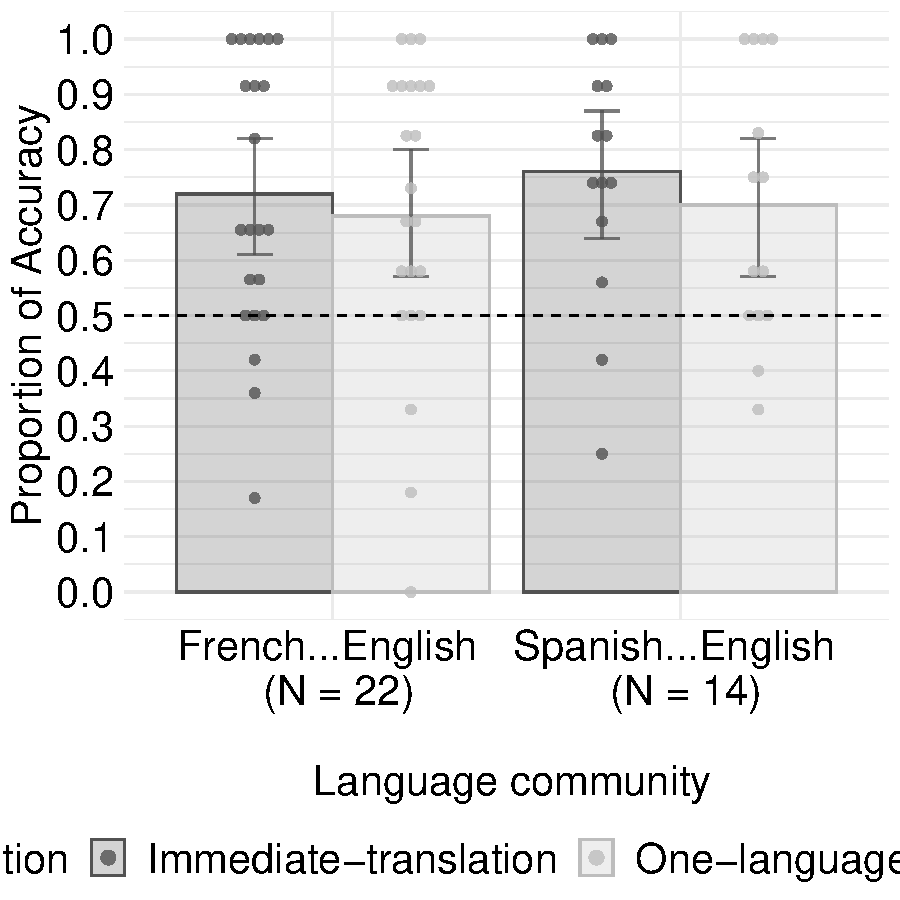
\includegraphics[width=0.6\linewidth]{TabletSwitch_supplemental_files/figure-latex/FigureS3-1} 

}

\caption{Average proportion of accuracy by condition and language community in the test blocks. Dots plot the data from each individual participant. Error bars indicate 95\% confidence intervals, and the black dashed line represents the at-chance accuracy level of 0.50.}\label{fig:FigureS3}
\end{figure}

\hypertarget{exploratory-analysis}{%
\subsubsection{Exploratory Analysis}\label{exploratory-analysis}}

\hypertarget{effect-of-age-1}{%
\paragraph{Effect of age}\label{effect-of-age-1}}

As an exploratory analysis, we also ran a logistic mixed-effects model with age as a fixed effect. Similar to the analysis on the sample reported in the main paper, model comparison with the model without age showed that adding age did not significantly improve the model (\(\chi^2\)(4) = 5.55, \(p\) = 0.24). Moreover, we had to prune the random slope for condition from the model since it would not converge, the final model specification was:

accuracy \textasciitilde{} condition * lang\_community * age\_in\_months + (1\textbar participant) + (1\textbar item)

\noindent The coefficient estimates from this model are shown in Table S7 and Figure S4 visualizes this model. The model did not reveal a significant effect of age, but there was a significant three-way condition * language community * age interaction. This was due to the crossover interaction in the French--English bilingual children, where their performance significantly improved on the \emph{immediate-translation} condition with age. In contrast, the Spanish--English children showed similar performance in the two conditions and across age.

\begin{table}[H]

\begin{center}
\begin{threeparttable}

\caption{\label{tab:unnamed-chunk-21}Table S7. Coefficient estimates from the logistic mixed-effects models predicting accuracy in the the test phase with age\_in\_months as an additional fixed effect.}

\begin{tabular}{lcccc}
\toprule
 & Estimate & $SE$ & $z$ & $p$\\
\midrule
Intercept & 1.060 & 0.235 & 4.490 & <.001\\
condition & -0.328 & 0.177 & -1.850 & 0.065\\
lang\_community & 0.236 & 0.420 & 0.562 & 0.574\\
age\_in\_months & 0.201 & 0.192 & 1.050 & 0.295\\
condition * lang\_community & -0.054 & 0.354 & -0.153 & 0.878\\
condition * age\_in\_months & -0.298 & 0.179 & -1.670 & 0.095\\
lang\_community * age\_in\_months & -0.286 & 0.383 & -0.747 & 0.455\\
condition * lang\_community * age\_in\_months & 0.975 & 0.357 & 2.730 & <.01\\
\bottomrule
\end{tabular}

\end{threeparttable}
\end{center}

\end{table}

\begin{figure}

{\centering 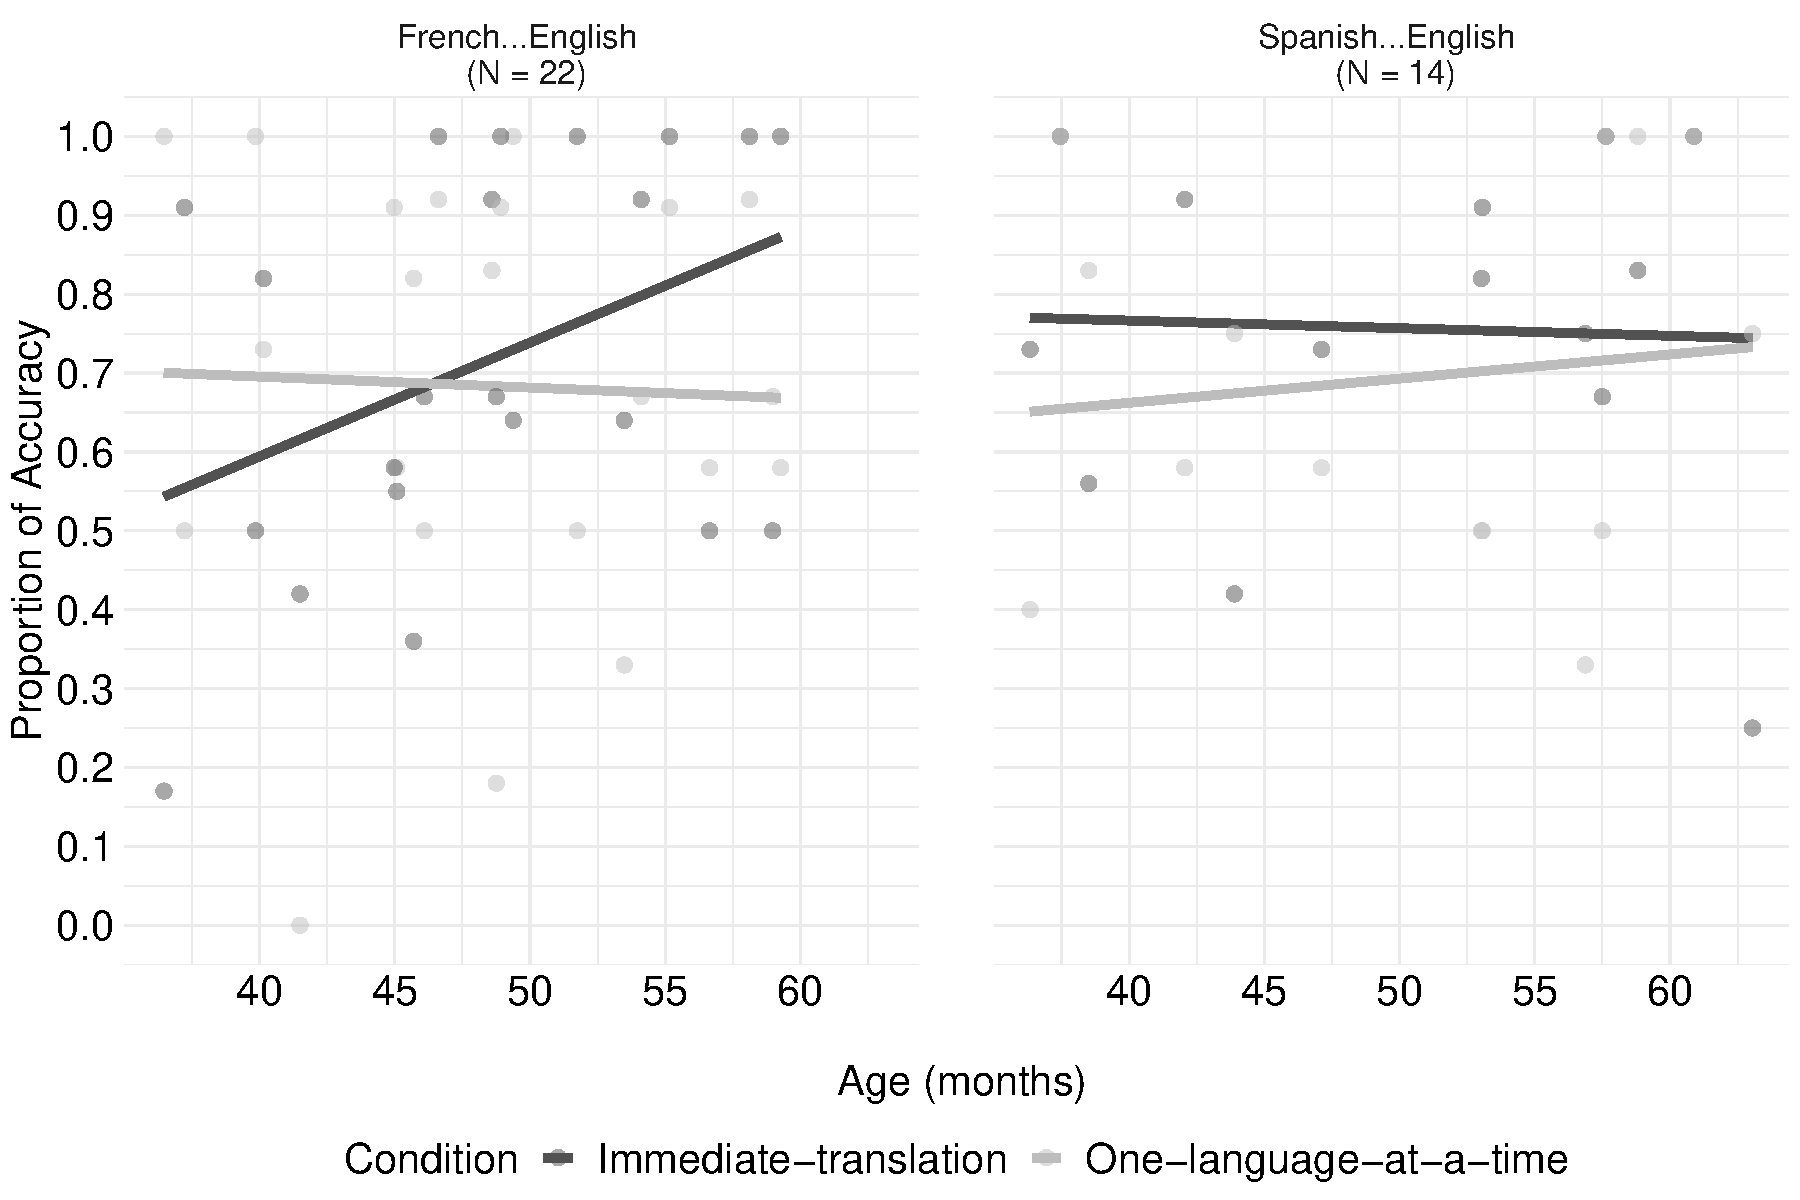
\includegraphics[width=0.9\linewidth]{TabletSwitch_supplemental_files/figure-latex/FigureS4-1} 

}

\caption{Proportion of accuracy by condition, language community, and age in the test phase. Individual dots plot the data from each individual participant.}\label{fig:FigureS4}
\end{figure}

\hypertarget{response-time-1}{%
\paragraph{Response time}\label{response-time-1}}

We also included response time on each correctly-responded test trial as a dependent variable. There were a total of 573 trials in this analysis. On average, French--English bilingual children had a mean response time of 2101ms in the \emph{immediate-translation} condition (\(SD\) = 1101.21; range = 451.86 -- 5130.5) and 1803ms in the \emph{one-language-at-a-time} condition (\(SD\) = 765.06; range = 339.33 -- 3101). On the other hand, Spanish--English bilingual children had a mean response time of 2410ms in the \emph{immediate-translation} condition (\(SD\) = 1108.38; range = 764.33 -- 4549) and 2033ms in the \emph{one-language-at-a-time} condition (\(SD\) = 1371.97; range = 457.25 -- 5525.8).

We ran a linear mixed-effects model with condition, language community, age, as well as their interactions, entered as fixed effects. A random slope of condition by participants and random intercepts of item were also entered. To correct issues of non-normality in response time, raw response time was log-transformed. The final model specification was:

log\_rt \textasciitilde{} condition * lang\_community * age\_in\_months + (1+ condition\textbar participant) + (1\textbar item)

\noindent The coefficient estimates from this model are shown in Table S8 and Figure S5 visualizes this model. Overall, visualization of the model suggests that, across both conditions and language communities, older children generally responded faster than younger children. However, the model did not reveal any significant effects or interactions of condition, language community, or age. Therefore, consistent to the patterns reported for the sample included in the main paper, in terms of response time, bilingual children in both communities performed similarly in word learning across both the \emph{immediate-translation} and \emph{one-language-at-a-time} conditions.

\begin{table}[H]

\begin{center}
\begin{threeparttable}

\caption{\label{tab:unnamed-chunk-24}Table S8. Coefficient estimates from the linear mixed-effects model predicting log-transformed response time in the test phase.}

\begin{tabular}{lcccc}
\toprule
 & Estimate & $SE$ & $t$ & $p$\\
\midrule
Intercept & 7.180 & 0.085 & 84.800 & <.001\\
condition & -0.138 & 0.090 & -1.530 & 0.137\\
lang\_community & 0.066 & 0.168 & 0.394 & 0.696\\
age\_in\_months & -0.129 & 0.082 & -1.570 & 0.126\\
condition * lang\_community & -0.171 & 0.180 & -0.953 & 0.349\\
condition * age\_in\_months & 0.036 & 0.089 & 0.403 & 0.69\\
lang\_community * age\_in\_months & 0.076 & 0.164 & 0.466 & 0.644\\
condition * lang\_community * age\_in\_months & -0.189 & 0.178 & -1.060 & 0.298\\
\bottomrule
\end{tabular}

\end{threeparttable}
\end{center}

\end{table}

\begin{figure}

{\centering 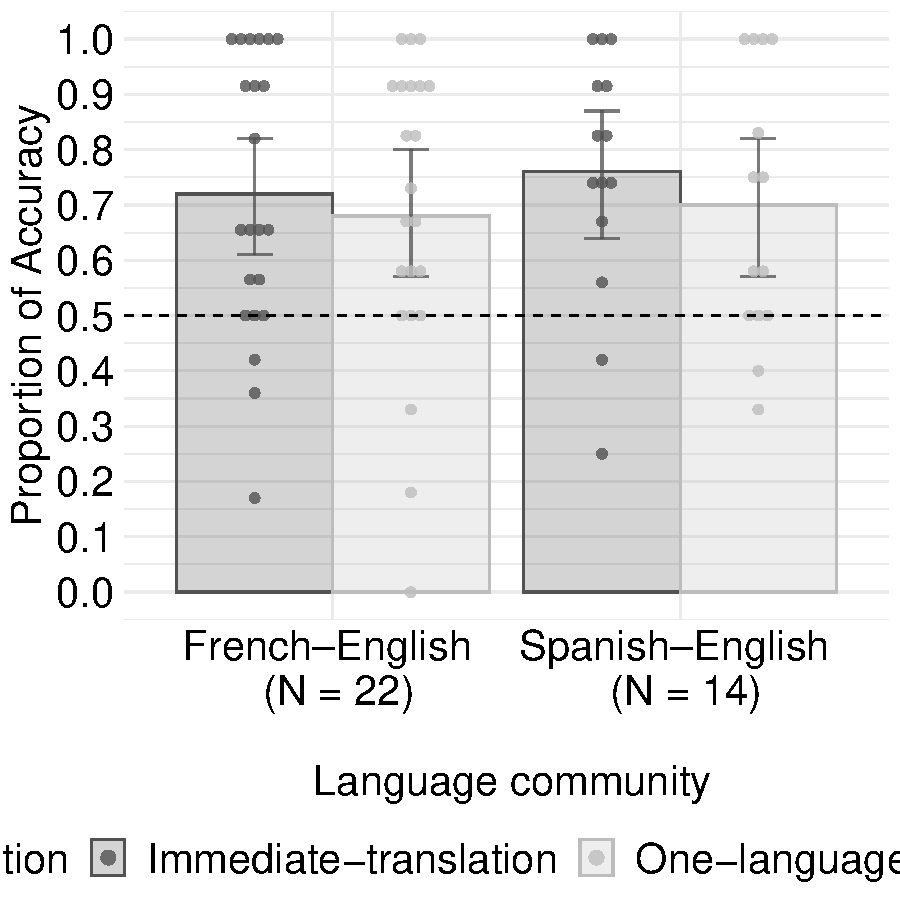
\includegraphics[width=0.9\linewidth]{TabletSwitch_supplemental_files/figure-latex/FigureS5-1} 

}

\caption{Response time by condition, language community, and age in the test phase. Individual dots plot the data from each individual participant.}\label{fig:FigureS5}
\end{figure}

\hypertarget{language-proficiency-in-all-participants}{%
\paragraph{Language proficiency in all participants}\label{language-proficiency-in-all-participants}}

For a more inclusive analysis on the effect of proficiency, this analysis also included data from children who were previously eliminated for not fulfilling the language criteria --- either the criteria reported in the main paper or the more stringent criteria reported in this document. In total, there were 30 French--English children and 22 Spanish--English children who were born full term and without any reported language problems or participated without any problem. Among this group of children, the French--English children had a mean proficiency score of 8.42 (\(SD\) = 1.93, range = 3 -- 10) and the Spanish--English children had a mean proficiency score of 8.34 (\(SD\) = 2.07, range = 2 -- 10). To explore the effect of proficiency, we added a variable of proficiency score to the logistic mixed-effects model. The initial model specification was:

accuracy \textasciitilde{} condition * lang\_community * proficiency + (1+ condition\textbar participant) + (1\textbar item)

However, as the initial model could not converge, we removed the random slope for condition and the random intercept for stimulus item. Moreover, since we did not find any significant difference between the two communities in the main accuracy analysis, we further pruned the effect of language community from the model. Note that model comparison between the model with language community and the one without also indicated no significant improvement in model fit, \(\chi^2\)(4) = 7.44, \emph{p} = 0.12. Therefore, the final model was:

accuracy \textasciitilde{} condition * proficiency + (1\textbar participant)

The coefficient estimates from this model are shown in Table S9 and Figure S6 visualizes this model. The model revealed a significant effect of proficiency, suggesting that bilingual children were overall more accurate for trials in which they had a higher level of language proficiency in the trial language. In contrast to the patterns reported for the sample included in the main paper, this model here revealed that the effect of proficiency may be more evident when a wider range of language proficiency level was included in the analysis. In other words, the sample reported in the main paper could have possibly focused on children who were relatively proficient. Yet, the lack of a significant interaction points to the possibility that proficiency level did not affect children's accuracy in learning words under different language-switching patterns.

\begin{table}[H]

\begin{center}
\begin{threeparttable}

\caption{\label{tab:unnamed-chunk-27}Table S9. Coefficient estimates from the logistic mixed-effects model predicting accuracy in the test phase with proficiency scores among all the children.}

\begin{tabular}{lcccc}
\toprule
 & Estimate & $SE$ & $z$ & $p$\\
\midrule
Intercept & 0.109 & 0.416 & 0.261 & 0.794\\
condition & -0.428 & 0.596 & -0.717 & 0.473\\
proficiency & 0.121 & 0.046 & 2.630 & <.01\\
condition * proficiency & 0.049 & 0.070 & 0.699 & 0.485\\
\bottomrule
\end{tabular}

\end{threeparttable}
\end{center}

\end{table}

\begin{figure}

{\centering 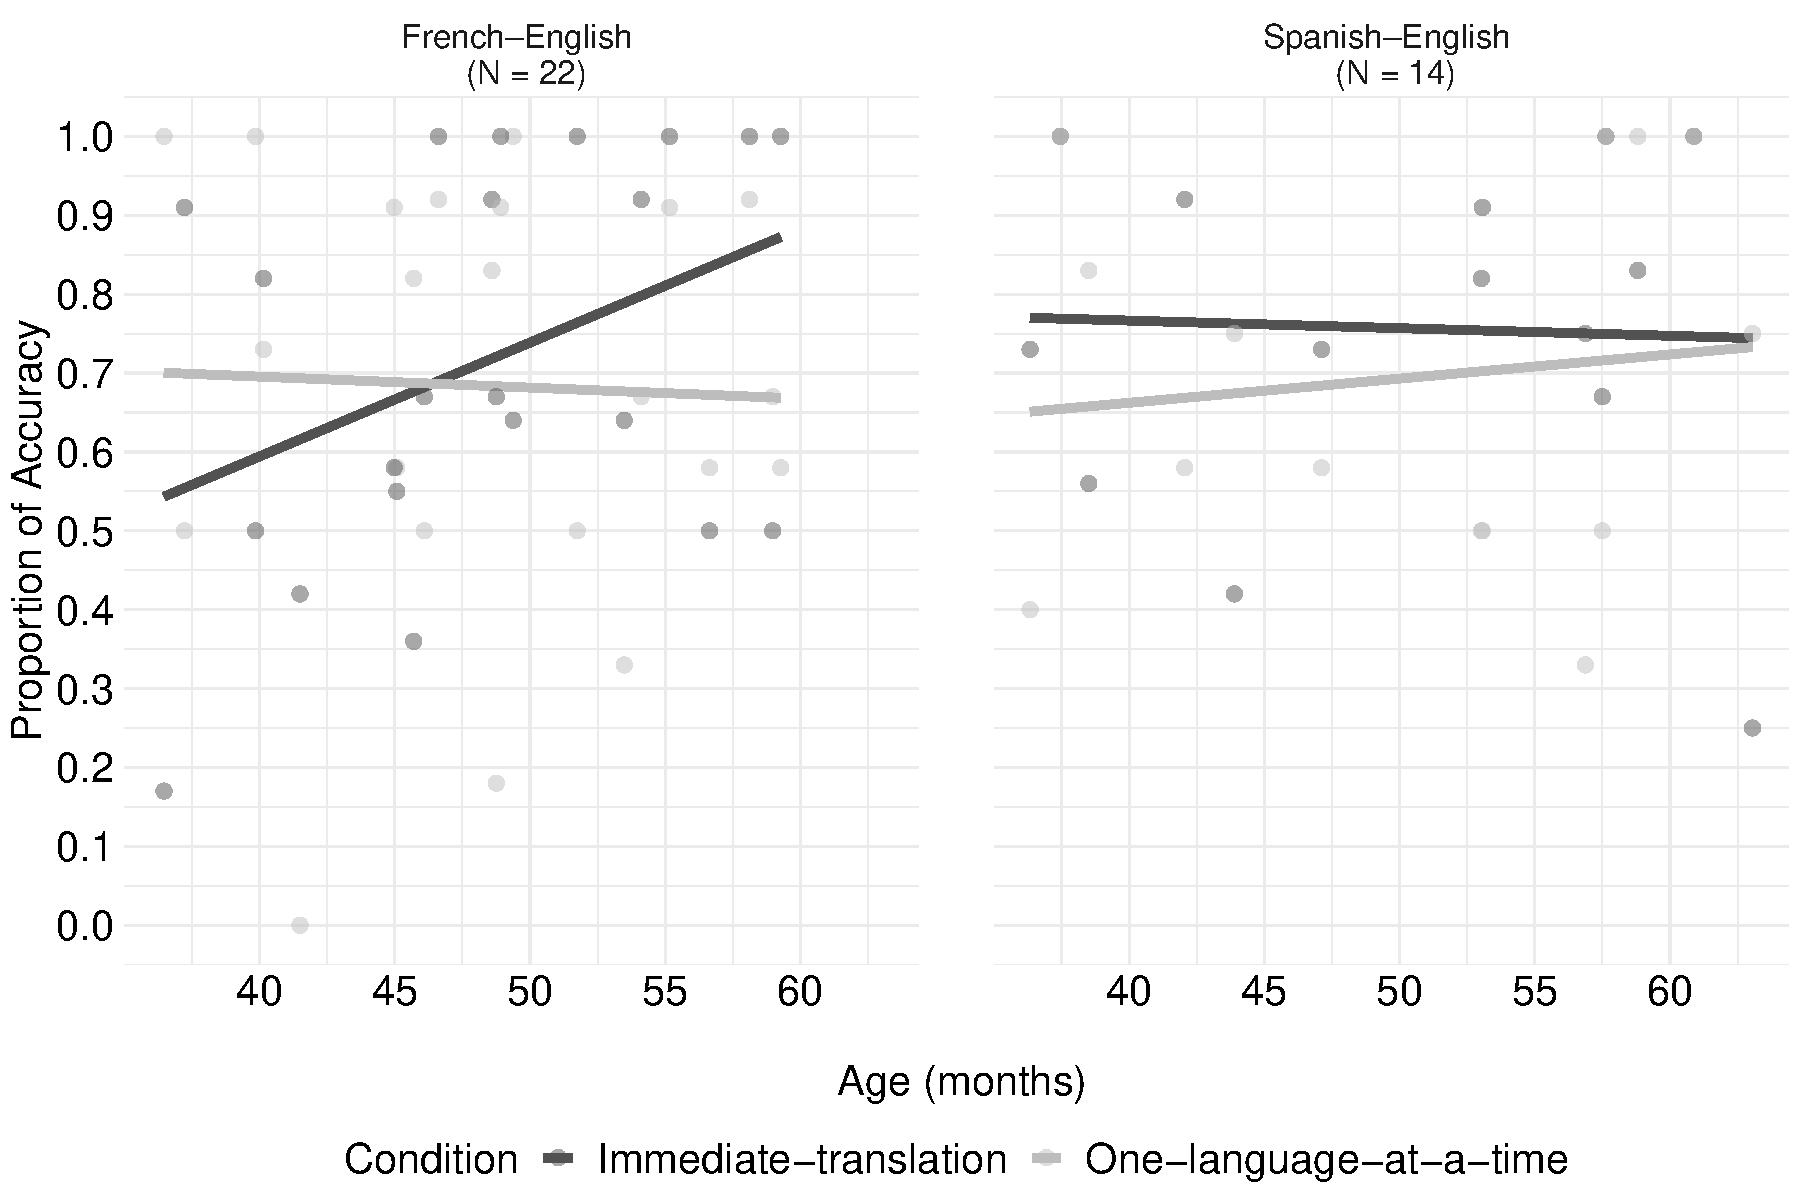
\includegraphics[width=0.5\linewidth]{TabletSwitch_supplemental_files/figure-latex/FigureS6-1} 

}

\caption{Proportion of accuracy of all children by condition and proficiency in the test blocks. Individual dots plots the data from each individual participant.}\label{fig:FigureS6}
\end{figure}


\end{document}
